\begin{lstlisting}[float=p,label=lst:sdg-calls,
  caption={Program with calls resulting in the SDG in \autoref{fig:sdg-calls}}]
class Main {
  static int global = 1;
  
  public static void main(String[] args) {
    boolean res1 = foo(42);
    int res2 = bar(res1);
    System.out.println(res2);
  }
  
  private static boolean foo(int n) {
    if(n < global)
      return false;
    gloabl = n;
    return true;
  }
  
  private static int bar(boolean b) {
    if(b)
      return 2;
    return 3;
  }
}
\end{lstlisting}

\begin{figure}[p]
  \centering
    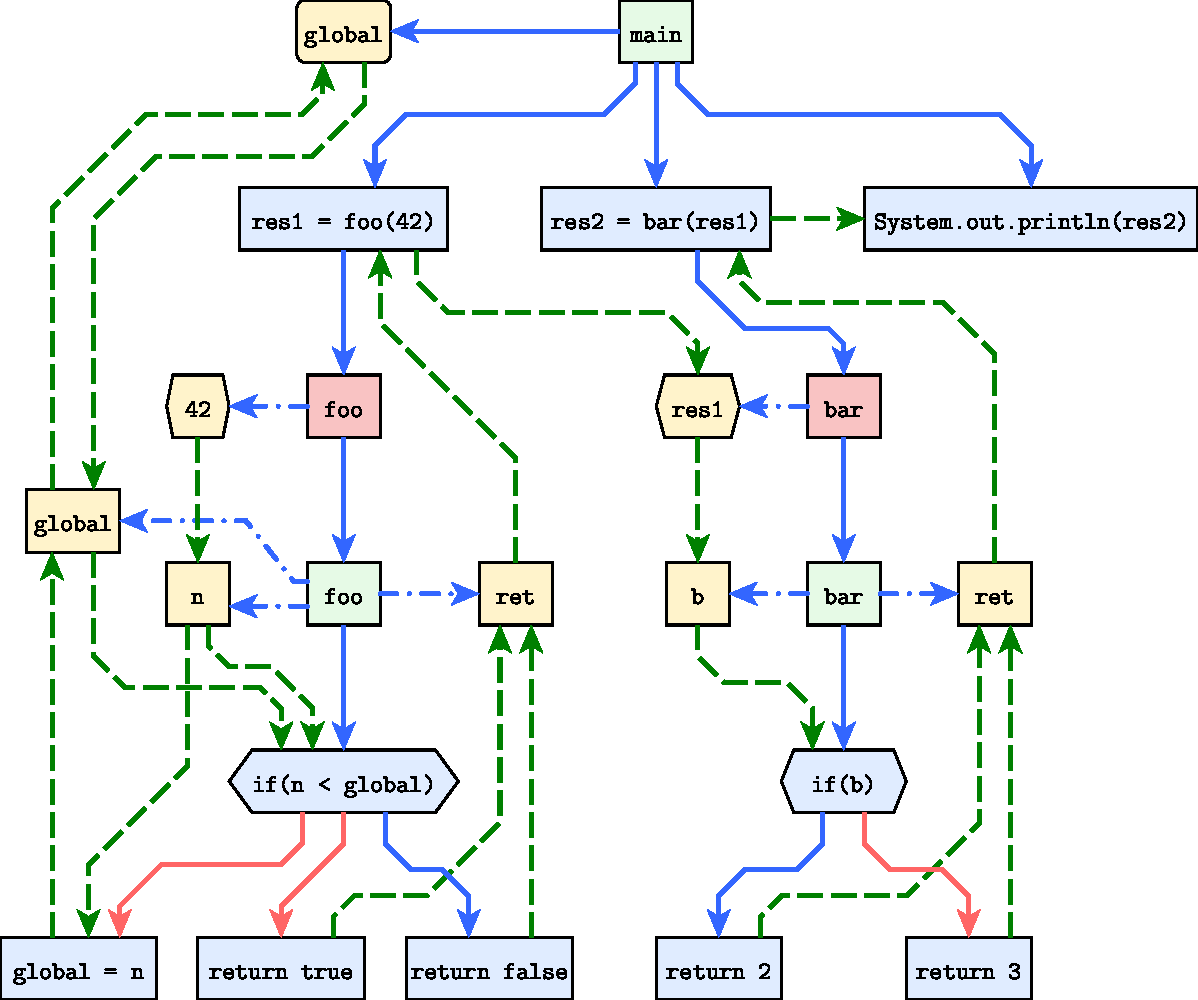
\includegraphics[scale=0.6]{sdgs/calls}
  \caption{SDG for the sample program in \autoref{lst:sdg-calls}}
  \label{fig:sdg-calls}
\end{figure}
